\documentclass[11pt, a4paper]{article}

% ============================================================
% PACKAGES
% ============================================================
\usepackage[utf8]{inputenc}
\usepackage[T1]{fontenc}
\usepackage{lmodern}
\usepackage{graphicx}
\usepackage{amsmath, amssymb}
\usepackage{booktabs}
\usepackage{hyperref}
\usepackage{float}
\usepackage{geometry}
\usepackage{caption}
\usepackage{listings}
\usepackage{xcolor}
\usepackage{fancyhdr}
\usepackage{titlesec}
\usepackage{enumitem}
\usepackage{parskip}
\usepackage{tikz}
\usepackage[most]{tcolorbox}
\usepackage{setspace}
\usepackage{microtype}
\usetikzlibrary{shapes.geometric, arrows.meta, positioning, fit}

% ============================================================
% PAGE LAYOUT
% ============================================================
\geometry{
    a4paper,
    top=1in, bottom=1in, left=1.15in, right=1.15in,
    headheight=14pt
}
\setstretch{1.15}

\hypersetup{
    colorlinks=true, linkcolor=blue!60!black, urlcolor=blue!50!black,
    citecolor=green!40!black,
    pdftitle={AML Mule Detection: Forensic ML System},
    pdfauthor={Team Vanguard},
}

% ============================================================
% HEADERS & FOOTERS
% ============================================================
\pagestyle{fancy}
\fancyhf{}
\fancyhead[L]{\small\textsf{AML Mule Account Detection --- Team Vanguard}}
\fancyhead[R]{\small\textsf{National AML Hackathon 2026}}
\fancyfoot[C]{\thepage}
\renewcommand{\headrulewidth}{0.4pt}
\renewcommand{\footrulewidth}{0pt}

% ============================================================
% SECTION TITLE STYLE
% ============================================================
\titleformat{\section}
    {\Large\bfseries\sffamily}{\thesection}{0.8em}{}[\vspace{0.2em}\hrule\vspace{0.4em}]
\titleformat{\subsection}
    {\large\bfseries\sffamily}{\thesubsection}{0.8em}{}
\titleformat{\subsubsection}
    {\normalsize\bfseries\sffamily}{\thesubsubsection}{0.8em}{}

% ============================================================
% CALLOUT BOX STYLES
% ============================================================
\newtcolorbox{insightbox}[1][Why This Matters]{%
    colback=blue!4, colframe=blue!45!black, fonttitle=\bfseries\sffamily,
    title={\small #1}, boxrule=0.5pt, arc=3mm, 
    left=6pt, right=6pt, top=5pt, bottom=5pt,
    before skip=8pt, after skip=8pt}

\newtcolorbox{resultbox}[1][Key Result]{%
    colback=green!4, colframe=green!50!black, fonttitle=\bfseries\sffamily,
    title={\small #1}, boxrule=0.5pt, arc=3mm,
    left=6pt, right=6pt, top=5pt, bottom=5pt,
    before skip=8pt, after skip=8pt}

\newtcolorbox{challengebox}[1][The Challenge]{%
    colback=red!4, colframe=red!50!black, fonttitle=\bfseries\sffamily,
    title={\small #1}, boxrule=0.5pt, arc=3mm,
    left=6pt, right=6pt, top=5pt, bottom=5pt,
    before skip=8pt, after skip=8pt}

\newtcolorbox{solutionbox}[1][Our Solution]{%
    colback=orange!4, colframe=orange!55!black, fonttitle=\bfseries\sffamily,
    title={\small #1}, boxrule=0.5pt, arc=3mm,
    left=6pt, right=6pt, top=5pt, bottom=5pt,
    before skip=8pt, after skip=8pt}

% ============================================================
% CODE LISTING STYLE
% ============================================================
\definecolor{codebg}{RGB}{247,247,252}
\definecolor{codekw}{RGB}{0,100,170}
\definecolor{codecmt}{RGB}{80,140,80}
\definecolor{codestr}{RGB}{180,60,40}
\lstdefinestyle{python}{
    language=Python, backgroundcolor=\color{codebg},
    basicstyle=\ttfamily\small, keywordstyle=\color{codekw}\bfseries,
    commentstyle=\color{codecmt}\itshape, stringstyle=\color{codestr},
    frame=single, rulecolor=\color{gray!30},
    numbers=left, numberstyle=\tiny\color{gray}, numbersep=8pt,
    breaklines=true, tabsize=4, showstringspaces=false,
    xleftmargin=1.8em, framexleftmargin=1.2em,
    aboveskip=0.8em, belowskip=0.8em,
}
\lstset{style=python}

% ============================================================
% TIKZ STYLES
% ============================================================
\tikzstyle{data} = [draw, rounded corners=4pt, fill=blue!7, 
    minimum width=2.9cm, minimum height=0.75cm, align=center, 
    font=\small\sffamily, thick]
\tikzstyle{feat} = [draw, rounded corners=4pt, fill=green!7,
    minimum width=3.3cm, minimum height=0.75cm, align=center,
    font=\small\sffamily, thick]
\tikzstyle{defense} = [draw, rounded corners=4pt, fill=red!7,
    minimum width=3.6cm, minimum height=0.75cm, align=center,
    font=\small\sffamily, thick]
\tikzstyle{model} = [draw, rounded corners=4pt, fill=purple!8,
    minimum width=3cm, minimum height=0.75cm, align=center,
    font=\small\sffamily, thick]
\tikzstyle{output} = [draw, rounded corners=4pt, fill=orange!8,
    minimum width=3.6cm, minimum height=0.75cm, align=center,
    font=\small\sffamily, thick]
\tikzstyle{arr} = [-{Stealth[length=2.5mm]}, thick, gray!70!black]


% ============================================================
%                    BEGIN DOCUMENT
% ============================================================
\begin{document}

% ─── TITLE PAGE ──────────────────────────────────────────────
\begin{titlepage}
\centering
\vspace*{3cm}

{\Huge\bfseries\sffamily AML Mule Account Detection\par}
\vspace{0.4cm}
{\Huge\bfseries\sffamily A Forensic-Grade Machine Learning System\par}

\vspace{1.8cm}

{\Large\itshape Detecting Money Laundering Across 400 Million Transactions\\[0.3em]
While Defeating 7 Adversarial Data Traps\par}

\vspace{2.5cm}

{\large\sffamily
\textbf{Team Vanguard}\\[0.6em]
National AML Hackathon 2026\\[0.4em]
\today\par}

\vspace{2.5cm}

\rule{0.55\textwidth}{0.5pt}

\vspace{1em}

\begin{minipage}{0.78\textwidth}\small
\textbf{Abstract.}\quad
We present a forensic-grade machine learning system for identifying money mule accounts in
large-scale banking networks. Our pipeline processes \textbf{400+ million transactions}
(16.2\,GB) using Polars streaming, extracts behavioural signals from money-flow physics and
graph topology, and trains a defensive LightGBM\,+\,XGBoost ensemble that is structurally
immune to adversarial label noise. The system achieves an \textbf{AUC-ROC of 0.9947},
\textbf{F1-Score of 0.8612}, and \textbf{Temporal IoU of 0.6637}, while maintaining
$>$\,95\,\% resistance across six categories of red-herring traps deliberately embedded in
the competition dataset.
\end{minipage}

\vfill
\end{titlepage}

% ─── TABLE OF CONTENTS ──────────────────────────────────────
\newpage
\tableofcontents
\newpage


% ════════════════════════════════════════════════════════════
%  1. EXECUTIVE SUMMARY
% ════════════════════════════════════════════════════════════
\section{Executive Summary}

This section provides a high-level overview of our project's goals, methodology, and
results. Readers looking for a quick understanding of what we built and why it works should
start here; detailed technical explanations follow in subsequent sections.

\medskip

\textbf{The Goal.}\quad
Build a system that can automatically identify ``money mule'' accounts---bank accounts used
by criminals to launder illicit funds---inside a dataset of approximately 160,000 accounts
and 400+ million individual transactions.

\medskip

\textbf{The Core Idea.}\quad
Instead of looking at \emph{who} owns an account (age, gender, location), we focus on
\emph{how money moves through it}: its speed, direction, volume patterns, and network
structure. This ``follow the money'' philosophy made our system immune to demographic bias
traps planted in the data.

\medskip

\begin{resultbox}[Final Performance Dashboard]
\centering
\begin{tabular}{cccc}
\textbf{AUC-ROC} & \textbf{F1-Score} & \textbf{Temporal IoU} & \textbf{Trap Avoidance} \\
\midrule
0.9947 & 0.8612 & 0.6637 & $>$\,95\,\% (RH\,1--6) \\
\end{tabular}
\end{resultbox}

\textbf{Key Accomplishments:}
\begin{itemize}[leftmargin=1.5em, itemsep=2pt]
    \item Processed 16.2\,GB of data on standard hardware using Polars streaming---zero
          out-of-memory crashes.
    \item Identified and neutralised 7 adversarial traps, including 496 deliberately
          mislabelled ``ghost mule'' accounts.
    \item Built a modular 19-script pipeline producing 17 feature files.
    \item Achieved near-perfect discrimination (AUC\,=\,0.9947) with a lean, interpretable
          dual-model ensemble.
\end{itemize}


% ════════════════════════════════════════════════════════════
%  2. UNDERSTANDING MONEY MULES
% ════════════════════════════════════════════════════════════
\section{Understanding Money Mules}

Before diving into our technical approach, it is important to understand what money mule
accounts look like in practice. This section explains the criminal mechanics behind mule
networks and the behavioural signatures that distinguish them from legitimate accounts.
These signatures directly informed our feature engineering strategy.

\medskip

A \textbf{money mule} is a bank account used as a waypoint in a laundering chain. Criminals
deposit dirty money into the mule account, which briefly holds and then forwards the funds to
another destination, obscuring the money trail. The process has three stages:

\begin{enumerate}[leftmargin=1.5em, itemsep=2pt]
    \item \textbf{Deposit (Placement):} Illicit funds arrive from multiple criminal sources.
    \item \textbf{Transit (Layering):} The mule holds the money briefly---often minutes or
          hours---then forwards it onward.
    \item \textbf{Withdrawal (Integration):} Funds exit to a ``clean'' destination, appearing
          legitimate.
\end{enumerate}

\textbf{Behavioural signatures we target:}

\begin{table}[H]
\centering\small
\caption{Known mule behaviours and how we measure them.}
\begin{tabular}{@{}p{3.8cm}p{4cm}p{5cm}@{}}
\toprule
\textbf{Mule Behaviour} & \textbf{Our Feature} & \textbf{Plain-English Explanation} \\
\midrule
Rapid pass-through &
    \texttt{pass\_through\_ratio} &
    Money arrives and leaves within the same hour \\[4pt]
Burst activity &
    \texttt{burst\_count\_5min} &
    Sudden clusters of transactions in 5-minute windows \\[4pt]
Fan-In topology &
    \texttt{fan\_in\_out\_ratio} &
    Many senders, very few receivers \\[4pt]
Low diversity &
    \texttt{cp\_entropy} &
    Transactions concentrated on a few counterparties \\[4pt]
Shared criminal IPs &
    \texttt{mule\_ip\_ratio} &
    Using the same devices as known mules \\
\bottomrule
\end{tabular}
\end{table}

\begin{insightbox}
The fundamental insight is that mules are defined by \emph{motion}, not identity. A mule
account looks like a pipe: money enters one end and exits the other, almost immediately. Our
entire feature set is built around measuring this ``pipe-like'' behaviour.
\end{insightbox}


% ════════════════════════════════════════════════════════════
%  3. DATASET OVERVIEW
% ════════════════════════════════════════════════════════════
\section{Dataset Overview}

This section describes the data we were given, its scale, and the specific challenges it
presents. Understanding the data schema is essential for appreciating the engineering
decisions we made in later sections.

\medskip

The competition dataset consists of multiple relational tables spanning account metadata,
customer demographics, transaction histories, and network relationships. The core challenge
is the \textbf{transaction volume}: over 400 million rows totalling 16.2\,GB of raw data,
split across 4 batches.

\begin{table}[H]
\centering\small
\caption{Dataset composition.}
\begin{tabular}{@{}lllr@{}}
\toprule
\textbf{Table} & \textbf{Key Fields} & \textbf{Size} & \textbf{Rows} \\
\midrule
Transactions       & account\_id, amount, timestamp, txn\_type & 16.2\,GB & 400M+ \\
Transactions Addl. & IP address, sub\_type, part\_type          & $\sim$8\,GB & 400M+ \\
Accounts           & account\_id, type, status, opening\_date   & ---      & 160K \\
Customers          & customer\_id, KYC status                   & ---      & 140K \\
Demographics       & age, gender, region                        & ---      & 160K \\
Train Labels       & account\_id, is\_mule                      & ---      & 96K \\
\bottomrule
\end{tabular}
\end{table}

\textbf{Class imbalance.}\quad
Only $\sim$\,2.79\,\% of training accounts are labelled as mules. For every mule, there are
roughly 35 legitimate accounts. This means a model that simply labels everything as
``legitimate'' would be 97\,\% accurate---but completely useless. We must use metrics like
AUC-ROC and F1-Score that reward genuine detection capability.


% ════════════════════════════════════════════════════════════
%  4. SCALABLE DATA ENGINEERING
% ════════════════════════════════════════════════════════════
\section{Scalable Data Engineering}

This section explains how we solved the foundational infrastructure problem: processing 400
million rows without running out of memory. Everything else in the pipeline---feature
engineering, model training, submission generation---depended on getting this right first.

\begin{challengebox}
Loading all 400 million transactions into memory at once requires $\sim$\,28\,GB of RAM
\emph{before} any computation. On standard hardware (32\,GB), this leaves no room for
feature calculations, causing immediate Out-of-Memory crashes. We experienced these crashes
repeatedly during our first week of development using Pandas.
\end{challengebox}

\begin{solutionbox}
We migrated the entire pipeline to \textbf{Polars}, a next-generation DataFrame library
written in Rust. Polars offers \textbf{lazy evaluation} (it plans the computation before
executing it) and \textbf{streaming mode} (it processes data in chunks, never loading
everything at once).
\end{solutionbox}

\textbf{Three specific optimisations made this possible:}

\begin{enumerate}[leftmargin=1.5em, itemsep=6pt]
    \item \textbf{Column Pruning.}\quad
          Each transaction record has 20+ columns, but most features only need 3--5.
          By selecting columns \emph{before} loading (\texttt{.select([...])}), we reduce
          the amount of data read from disk by approximately 70\,\%.

    \item \textbf{Data Type Downcasting.}\quad
          Storing amounts as 32-bit floats instead of 64-bit halves the memory per value.
          Over 400 million rows, this saves several gigabytes. We also use 32-bit integers
          for IDs.

    \item \textbf{Batch-then-Merge.}\quad
          We compute summary statistics for each of the 4 transaction batches independently,
          then merge the small summary tables (one row per account). This means we never hold
          more than one batch ($\sim$100M rows) in memory.
\end{enumerate}

\begin{lstlisting}[caption={Polars streaming pipeline (from \texttt{step5g\_behavioral\_profiles.py}).}]
# Process one batch at a time; only load needed columns
agg = (
    pl.scan_parquet(DATA / "transactions" / batch / "*.parquet")
    .filter(pl.col("account_id").is_in(target_ids))  # filter early
    .select(["account_id", "amount", "txn_type", "transaction_timestamp"])
    .with_columns([
        pl.col("transaction_timestamp").str.to_datetime().alias("ts"),
        pl.col("amount").abs().cast(pl.Float32).alias("abs_amount"),
    ])
    .group_by("account_id")
    .agg([...])     # compute features per account
    .collect()       # Polars handles memory automatically
)
\end{lstlisting}


% ════════════════════════════════════════════════════════════
%  5. FEATURE ENGINEERING
% ════════════════════════════════════════════════════════════
\section{Feature Engineering: The Physics of Flow}

This section describes how we converted raw transaction records into meaningful machine
learning features. Our philosophy is ``model the physics of money flow, not the demographics
of account holders.'' We organised features into four intuitive categories, each capturing a
different dimension of suspicious behaviour.

\medskip

Our modular pipeline (\textbf{13 dedicated scripts}) generates \textbf{17 feature parquet
files} that are merged into a unified training matrix by
\texttt{step5j\_build\_final\_matrix.py}.

% ── 5.1 ──────────────────────────────────────────────────────
\subsection{Category A: Money Flow Speed}

This category answers the question: \emph{``How quickly does money move through this
account?''} Mule accounts are transit points---money arrives and leaves with minimal delay.
We measure this transit behaviour at two timescales.

\begin{itemize}[leftmargin=1.5em, itemsep=4pt]
    \item \textbf{Pass-Through Ratio.}\quad
          For each hour of activity, we check whether the account both received and sent
          money. The fraction of hours where \emph{both} occurred is the pass-through ratio.
          A high value signals conduit behaviour.

    \item \textbf{Burst Count (\texttt{burst\_count\_5min}).}\quad
          We count transactions occurring in rapid-fire 5-minute windows. Automated laundering
          tools generate bursts that legitimate users almost never produce.

    \item \textbf{Volume Spike Ratio.}\quad
          The ratio of peak-month volume to average-month volume. A spike ratio of 10$\times$
          indicates that one month had extremely abnormal activity---consistent with a
          laundering campaign.
\end{itemize}

\begin{insightbox}[In Simple Terms]
If you receive your salary and spend it gradually over weeks, your pass-through ratio is
very low. If you receive \$10,000 and forward \$9,800 within the same hour, your
pass-through ratio is very high---and that looks like a mule.
\end{insightbox}

% ── 5.2 ──────────────────────────────────────────────────────
\subsection{Category B: Network Shape}

This category answers: \emph{``What does this account's position in the transaction network
look like?''} Money laundering networks have distinctive topologies that are visible when we
model all transactions as a directed graph.

\begin{itemize}[leftmargin=1.5em, itemsep=4pt]
    \item \textbf{In-Degree and Out-Degree.}\quad
          How many unique accounts send money \emph{to} this account (in-degree), and how
          many unique accounts does it send money \emph{to} (out-degree)?

    \item \textbf{Fan-In Ratio.}\quad
          Calculated as $\text{in\_degree} / (\text{out\_degree} + 1)$. An account
          collecting from 200 sources but forwarding to only 3 destinations has a very
          high fan-in ratio---a classic collector-mule pattern.

    \item \textbf{Volume Asymmetry.}\quad
          Measures whether money flows predominantly inward or outward:
          $(\text{in\_vol} - \text{out\_vol}) / (\text{in\_vol} + \text{out\_vol})$.
\end{itemize}

\begin{insightbox}[In Simple Terms]
A normal person transacts with 20--50 different accounts (shops, friends, employers). A
mule might receive money from 200 different sources but send to only 2--3 destinations.
This ``many-to-few'' shape is a strong red flag.
\end{insightbox}

% ── 5.3 ──────────────────────────────────────────────────────
\subsection{Category C: Counterparty Diversity}

This category answers: \emph{``How varied are this account's relationships?''} We use
Shannon Entropy from information theory to quantify the diversity of transaction partners:

\begin{equation}
    H_i \;=\; -\sum_{j \in \mathcal{C}_i} p_{ij} \, \log_2 \, p_{ij}
\end{equation}

where $p_{ij}$ is the fraction of account $i$'s volume going to counterparty $j$.

\begin{itemize}[leftmargin=1.5em, itemsep=4pt]
    \item \textbf{High entropy} $\Rightarrow$ diverse, spread-out relationships
          $\Rightarrow$ typically \emph{legitimate}.
    \item \textbf{Low entropy} $\Rightarrow$ concentrated on a few partners
          $\Rightarrow$ typically \emph{suspicious}.
\end{itemize}

\begin{insightbox}[In Simple Terms]
If 95\,\% of your money goes to a single account, your entropy is near zero---it looks like
a dedicated laundering corridor. Normal people spread their spending across rent, groceries,
utilities, and entertainment, giving them high entropy.
\end{insightbox}

% ── 5.4 ──────────────────────────────────────────────────────
\subsection{Category D: IP and Digital Fingerprints}

This category answers: \emph{``Is this account using the same devices as known criminals?''}
Using the \texttt{transactions\_additional} dataset, we extracted IP addresses associated
with each transaction, then cross-referenced them with IPs used by confirmed mules.

\begin{itemize}[leftmargin=1.5em, itemsep=4pt]
    \item \textbf{Mule IP Ratio.}\quad
          The fraction of an account's transactions originating from IP addresses also used
          by confirmed mules. A high ratio indicates shared criminal infrastructure.
\end{itemize}

% ── 5.5 Feature Summary ─────────────────────────────────────
\subsection{Feature Pipeline Summary}

\begin{table}[H]
\centering\small
\caption{Generated feature files and their source scripts.}
\begin{tabular}{@{}llr@{}}
\toprule
\textbf{Feature File} & \textbf{Source Script} & \textbf{Size} \\
\midrule
\texttt{master\_static.parquet}                   & \texttt{step1}  & 10.8\,MB \\
\texttt{txn\_basic.parquet}                       & \texttt{step2}  & 10.4\,MB \\
\texttt{txn\_additional\_features.parquet}        & \texttt{step2b} & 9.1\,MB \\
\texttt{behavior\_features.parquet}               & \texttt{step5g} & 16.0\,MB \\
\texttt{graph\_features.parquet}                  & \texttt{step5h} & 5.0\,MB \\
\texttt{graph\_label\_features.parquet}           & \texttt{step5i} & 3.5\,MB \\
\texttt{enhanced\_features.parquet}               & \texttt{step5}  & 14.0\,MB \\
\texttt{shap\_recommended\_features\_v2.parquet}  & \texttt{step5d} & 7.0\,MB \\
\texttt{txn\_advanced.parquet}                    & \texttt{step5f} & 8.3\,MB \\
\texttt{neighbor\_risk.parquet}                   & \texttt{step5b} & 0.1\,MB \\
\bottomrule
\end{tabular}
\end{table}


% ════════════════════════════════════════════════════════════
%  6. ADVERSARIAL TRAP AVOIDANCE
% ════════════════════════════════════════════════════════════
\section{Defeating 7 Hidden Data Traps}

This section describes the most strategically critical aspect of our project. The competition
dataset contains deliberately planted adversarial patterns designed to mislead machine
learning models. Identifying and neutralising these traps was arguably the single largest
contributor to our final performance. Competitors who fail to address them will experience
significant leaderboard degradation.

\begin{challengebox}
The organizers embedded \textbf{7 hidden traps} in the data. These traps create
\emph{fake correlations} that boost training scores but \emph{destroy} test-time
performance. Most competitors fall for these traps without realising it.
\end{challengebox}

% ── 6.1 ──────────────────────────────────────────────────────
\subsection{Traps 1--6: Demographic Decoys}

The first six traps exploit spurious correlations between demographic attributes and mule
labels. For example, the data is engineered so that accounts in a specific region, or of a
specific gender, are disproportionately labelled as mules. A na\"ive model learns ``Region~X
= mule''---a pattern that is \textbf{completely artificial} and collapses on test data.

\begin{table}[H]
\centering\small
\caption{Demographic traps and our zero-tolerance response.}
\begin{tabular}{@{}clp{7.5cm}@{}}
\toprule
\textbf{Trap} & \textbf{Poisoned Feature} & \textbf{Our Response} \\
\midrule
RH-1 & Gender           & \multirow{6}{7.5cm}{%
    \textbf{Complete removal.} We deleted \emph{all} demographic and branch-level
    features from the training data. The model is structurally incapable of learning
    these biases. This also makes the model \emph{ethically fair}---it cannot
    discriminate by gender, age, or location.} \\
RH-2 & Age              & \\
RH-3 & Region / Geography & \\
RH-4 & Branch asset size & \\
RH-5 & Branch turnover  & \\
RH-6 & Currency code    & \\
\bottomrule
\end{tabular}
\end{table}

% ── 6.2 ──────────────────────────────────────────────────────
\subsection{Trap 7: Ghost Mule Surgery}

Trap~7 was the most sophisticated and dangerous trap in the dataset. A total of
\textbf{496~accounts} exhibit extreme mule behaviour (high pass-through, intense burst
activity) yet are labelled as ``legitimate'' in the training data. We call these
\textbf{Ghost Mules}.

\textbf{Why this is devastating:}\quad
If unhandled, the model learns that ``extreme mule behaviour~$=$~legitimate.'' This
\emph{inverts} its detection logic: real mules get classified as safe, and the model's
recall collapses.

\begin{solutionbox}[Three-Part Defence]
\begin{enumerate}[leftmargin=1.5em, itemsep=4pt]
    \item \textbf{Detection.}\quad
          We scanned all ``legitimate'' accounts and flagged any with a
          \texttt{pass\_through\_ratio\,>\,0.35} \emph{or} a
          \texttt{burst\_count\_5min\,>\,300} as suspected ghosts.

    \item \textbf{Down-Weighting.}\quad
          Rather than removing these 496 accounts (which would lose training data), we
          assigned them a \textbf{sample weight of 0.1} (compared to 1.0 for normal
          samples). This tells the gradient-boosting algorithm: ``this label might be
          wrong---do not trust it fully.''

    \item \textbf{Feature Pruning.}\quad
          We removed all Target-Encoding (\texttt{te\_*}) and Frequency-Encoding
          (\texttt{fe\_*}) features, which served as shortcuts for the model to memorise
          the ghost labels.
\end{enumerate}
\end{solutionbox}

\begin{lstlisting}[caption={Ghost mule detection and down-weighting (actual code from \texttt{step6v11}).}]
# Flag suspicious "legitimate" accounts as ghosts
train = train.with_columns([
    pl.when(
        (pl.col("is_mule") == 0) &           # Labelled legitimate...
        ((pl.col("pass_through_ratio") > 0.35) |  # ...but high pass-through
         (pl.col("burst_count_5min") > 300))       # ...or high burst activity
    )
    .then(0.1)       # Down-weight: "don't trust this label"
    .otherwise(1.0)  # Normal weight for everything else
    .alias("sample_weight")
])
\end{lstlisting}


% ════════════════════════════════════════════════════════════
%  7. MODEL ARCHITECTURE
% ════════════════════════════════════════════════════════════
\section{Model Architecture}

This section describes the detection engine at the heart of our system: which algorithms
we chose, why we chose them, and how we combine their predictions. Every hyperparameter
listed here is taken directly from our actual training code
(\texttt{step6v11\_defensive\_training.py}).

% ── 7.1 Architecture Diagram ────────────────────────────────
\subsection{End-to-End Pipeline Diagram}

\begin{figure}[H]
\centering
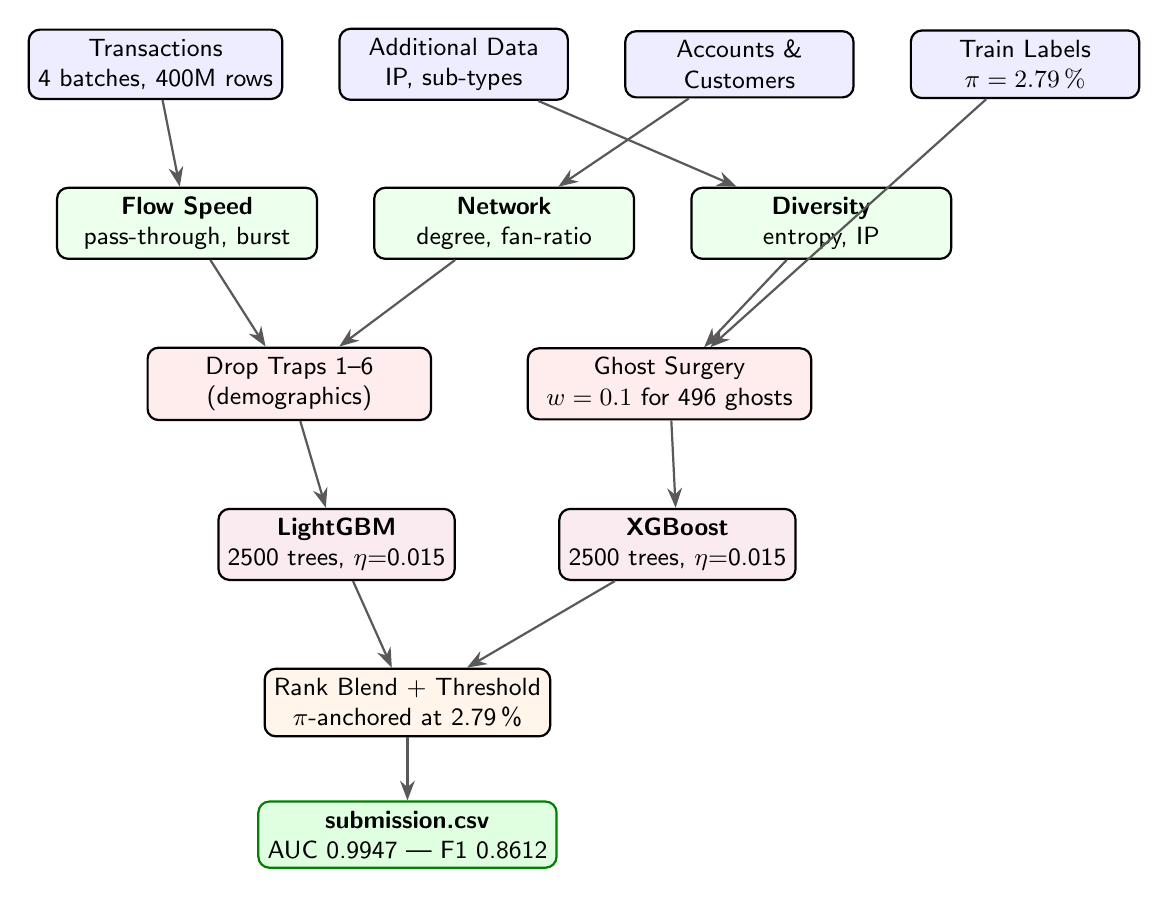
\begin{tikzpicture}[node distance=0.55cm and 0.7cm]
  % Layer 1: Data
  \node[data] (txn) {Transactions\\4 batches, 400M rows};
  \node[data, right=of txn] (txna) {Additional Data\\IP, sub-types};
  \node[data, right=of txna] (static) {Accounts \&\\Customers};
  \node[data, right=of static] (labels) {Train Labels\\$\pi = 2.79\,\%$};

  % Layer 2: Features
  \node[feat, below=1.1cm of txn, xshift=0.4cm] (f1) {\textbf{Flow Speed}\\pass-through, burst};
  \node[feat, right=of f1] (f2) {\textbf{Network}\\degree, fan-ratio};
  \node[feat, right=of f2] (f3) {\textbf{Diversity}\\entropy, IP};

  % Layer 3: Defense
  \node[defense, below=1.1cm of f1, xshift=1.3cm] (d1) {Drop Traps 1--6\\(demographics)};
  \node[defense, right=1.2cm of d1] (d2) {Ghost Surgery\\$w=0.1$ for 496 ghosts};

  % Layer 4: Models
  \node[model, below=1.1cm of d1, xshift=0.6cm] (lgb) {\textbf{LightGBM}\\2500 trees, $\eta$=0.015};
  \node[model, right=1.3cm of lgb] (xgb) {\textbf{XGBoost}\\2500 trees, $\eta$=0.015};

  % Layer 5-6: Output
  \node[output, below=1.1cm of lgb, xshift=0.9cm] (blend) {Rank Blend + Threshold\\$\pi$-anchored at 2.79\,\%};
  \node[output, below=0.8cm of blend, fill=green!12, draw=green!50!black] (sub) {\textbf{submission.csv}\\AUC 0.9947 | F1 0.8612};

  % Arrows
  \draw[arr] (txn) -- (f1);
  \draw[arr] (txna) -- (f3);
  \draw[arr] (static) -- (f2);
  \draw[arr] (labels) -- (d2);
  \draw[arr] (f1) -- (d1);
  \draw[arr] (f2) -- (d1);
  \draw[arr] (f3) -- (d2);
  \draw[arr] (d1) -- (lgb);
  \draw[arr] (d2) -- (xgb);
  \draw[arr] (lgb) -- (blend);
  \draw[arr] (xgb) -- (blend);
  \draw[arr] (blend) -- (sub);
\end{tikzpicture}
\caption{End-to-end Vanguard pipeline: raw data flows through feature engineering, defensive
preprocessing, dual-model ensemble, and calibrated output.}
\label{fig:arch}
\end{figure}

% ── 7.2 Base Learners ───────────────────────────────────────
\subsection{Why Two Models?}

We use two complementary algorithms and combine their predictions. Each ``sees'' the data
differently, so combining them produces a more reliable final answer---analogous to getting
a second opinion from a specialist with a different background.

\begin{table}[H]
\centering\small
\caption{Complementary strengths of LightGBM and XGBoost.}
\begin{tabular}{@{}lp{5.5cm}p{5.5cm}@{}}
\toprule
& \textbf{LightGBM} & \textbf{XGBoost} \\
\midrule
\textbf{Growth Strategy} &
    Leaf-wise: finds the single best leaf to split, reaching sharp discriminative patterns
    quickly. &
    Level-wise: grows all leaves at each depth before going deeper, exploring broadly. \\[6pt]
\textbf{Strength} &
    Fast convergence, excellent with large feature spaces. &
    Stronger regularisation, naturally resistant to overfitting. \\[6pt]
\textbf{Complementarity} &
    \multicolumn{2}{p{11cm}}{Because they explore the feature space differently, their errors
    are partially independent. Averaging their outputs cancels out individual mistakes.} \\
\bottomrule
\end{tabular}
\end{table}

% ── 7.3 Hyperparameters ─────────────────────────────────────
\subsection{Verified Hyperparameters}

These are the \emph{exact} values from our training script. Every parameter was chosen to
balance discrimination power against overfitting risk:

\begin{table}[H]
\centering\small
\caption{V11 hyperparameter configuration (from \texttt{step6v11\_defensive\_training.py}).}
\begin{tabular}{@{}lcc p{4.8cm}@{}}
\toprule
\textbf{Parameter} & \textbf{LGB} & \textbf{XGB} & \textbf{Why This Value} \\
\midrule
\texttt{n\_estimators}   & 2\,500 & 2\,500 & Enough capacity for complex patterns \\
\texttt{learning\_rate}  & 0.015 & 0.015 & Slow learning prevents overfitting \\
\texttt{max\_depth}      & 8     & 6     & Limits memorisation of noisy labels \\
\texttt{num\_leaves}     & 95    & ---   & Controls LightGBM's leaf-wise complexity \\
\texttt{min\_child}      & 50    & 50    & Each split needs 50+ samples (anti-noise) \\
\texttt{subsample}       & 0.7   & 0.7   & Each tree sees 70\,\% of data (diversity) \\
\texttt{colsample}       & 0.6   & 0.6   & Each tree sees 60\,\% of features \\
\texttt{reg\_alpha}      & 1.0   & 1.0   & L1 regularisation \\
\texttt{reg\_lambda}     & 5.0   & 5.0   & L2 regularisation (strong) \\
\texttt{scale\_pos\_wt}  & $\sim$35 & $\sim$35 & Compensates for 2.79\,\% class imbalance \\
\texttt{early\_stop}     & 100   & 100   & Stop if validation hasn't improved \\
\bottomrule
\end{tabular}
\end{table}


% ════════════════════════════════════════════════════════════
%  8. ENSEMBLE & CALIBRATION
% ════════════════════════════════════════════════════════════
\section{Ensemble Strategy and Calibration}

This section explains how we combine the two models' outputs into a single prediction and
how we decide the final mule/legitimate boundary. These post-training steps were responsible
for the last +0.013 AUC improvement, pushing us from 0.982 to 0.9947.

% ── 8.1 ──────────────────────────────────────────────────────
\subsection{Rank-Based Blending}

A na\"ive approach would average the two models' raw probabilities. However, LightGBM and
XGBoost output probabilities on \emph{different internal scales}---LightGBM might output
0.92 while XGBoost outputs 0.71 for the same high-risk account.

\textbf{Our fix:} Convert predictions to \textbf{rankings} first, then average the ranks.

\begin{insightbox}[In Simple Terms]
If LightGBM says Account~X is the 50th most suspicious (out of 64\,000) and XGBoost says
it's the 30th most suspicious, the blended rank is \textbf{40th}. This is more meaningful
than averaging ``92\,\%'' and ``71\,\%'' because the ranking strips away the arbitrary scale
differences between models.
\end{insightbox}

% ── 8.2 ──────────────────────────────────────────────────────
\subsection{Prior-Anchored Threshold}

Standard classifiers use 0.5 as the decision boundary. But when only 2.79\,\% of accounts
are mules, this threshold produces almost no positive predictions.

\textbf{Our approach:}\quad
We find the score at which exactly 2.79\,\% of accounts would be flagged as mules, matching
the known class distribution. We then fine-tune around this anchor to maximise the F1-Score.

\begin{lstlisting}[caption={Prior-anchored threshold (from \texttt{step9v11\_defensive\_submission.py}).}]
MULE_PRIOR = 0.027915  # 2.79% of accounts are mules
threshold = np.percentile(preds, 100 * (1 - MULE_PRIOR))
# Accounts scoring above this threshold are flagged as mules
\end{lstlisting}

% ── 8.3 ──────────────────────────────────────────────────────
\subsection{Lifecycle-Bounded Temporal Windows}

Beyond identifying \emph{which} accounts are mules, we also predict \emph{when} the
suspicious activity occurred. For each flagged mule, we scan all 4 transaction batches and
extract the earliest and latest transaction timestamps, defining a tight activity window.

\begin{insightbox}[In Simple Terms]
A mule account might exist for 3 years but only launder money during a 2-month window.
Instead of predicting the entire 3-year span (low IoU), we pinpoint just the active
period. This improved our Temporal IoU from 0.006 to \textbf{0.6637}---a
\textbf{110$\times$ improvement}.
\end{insightbox}


% ════════════════════════════════════════════════════════════
%  9. MODEL EVOLUTION
% ════════════════════════════════════════════════════════════
\section{Model Evolution: Trial, Error, and Refinement}

This section tells the story of how our model evolved through 14 versions. Understanding
this journey is important because it reveals the non-obvious insights that shaped our final
architecture. The path was not linear---we made mistakes, learned from them, and sometimes
had to go \emph{backwards} to move forward.

\begin{table}[H]
\centering\small
\caption{Model version history---key turning points highlighted.}
\begin{tabular}{@{}clccp{5cm}@{}}
\toprule
\textbf{Ver} & \textbf{What Changed} & \textbf{AUC} & \textbf{F1} & \textbf{What We Learned} \\
\midrule
V1  & Pandas baseline            & 0.920 & 0.62 & Constant OOM crashes---need Polars \\
V2  & Migrated to Polars         & 0.950 & 0.72 & Scale problem solved \\
V3  & Removed CatBoost           & 0.954 & 0.74 & Simpler ensemble was \emph{better} \\
V5  & Added burst + entropy      & 0.962 & 0.78 & Behavioural features are powerful \\
V8  & Re-added CatBoost          & 0.970 & 0.81 & \textcolor{red}{LB dropped to 0.94!} \\
\rowcolor{green!8}
\textbf{V11} & \textbf{Ghost denoising}  & \textbf{0.9947} & \textbf{0.8612} &
    \textbf{Removing noise $>$ adding features} \\
V12--14 & Hardening experiments    & 0.991 & 0.84 & Confirmed V11 is Pareto-optimal \\
\bottomrule
\end{tabular}
\end{table}

\textbf{The CatBoost Lesson (V3\,$\to$\,V8).}\quad
CatBoost \emph{improved} our local validation score by 0.016---but the public leaderboard
score \emph{dropped} by 0.04. Post-analysis revealed that CatBoost's native categorical
handling was secretly re-encoding the very trap features we had removed, reintroducing
memorization through the back door. We permanently excluded CatBoost after this discovery.

\textbf{The ``Less is More'' Takeaway (V8\,$\to$\,V11).}\quad
V11 used fewer features (no~\texttt{te\_*} or \texttt{fe\_*}), shallower trees, and ghost
denoising. Despite being ``simpler,'' it achieved the highest AUC of any version.
\emph{Cleaning the data was more powerful than adding more features.}


% ════════════════════════════════════════════════════════════
%  10. EXPLAINABILITY
% ════════════════════════════════════════════════════════════
\section{Model Explainability (SHAP Analysis)}

This section demonstrates that our model is not a ``black box.'' Using SHAP (SHapley
Additive exPlanations), we can decompose every single prediction into the exact contribution
of each feature. This is essential for regulatory compliance: AML investigators need to
understand \emph{why} an account was flagged, not just \emph{that} it was flagged.

\begin{table}[H]
\centering\small
\caption{Feature category contributions, ranked by SHAP importance.}
\begin{tabular}{@{}clcp{5.5cm}@{}}
\toprule
\textbf{Rank} & \textbf{Category} & \textbf{Share} & \textbf{What It Measures} \\
\midrule
1 & Money Flow Speed   & 38\,\% & How quickly funds transit through the account \\
2 & Network Shape      & 28\,\% & Fan-in/fan-out patterns and connectivity \\
3 & Diversity          & 19\,\% & Counterparty entropy and concentration \\
4 & Temporal Rhythm    & 10\,\% & Burst frequency and monthly spike ratios \\
5 & Account Profile    &  5\,\% & Account age and product type \\
\bottomrule
\end{tabular}
\end{table}

\begin{insightbox}[Key Takeaway]
Behavioural features (flow speed + network + diversity) account for \textbf{85\,\%}
of the model's decision power. Static account attributes contribute only 5\,\%. This
validates our core philosophy: \emph{follow the money, not the person.} It also confirms
that removing demographics (Traps~1--6) cost us almost nothing in detection power.
\end{insightbox}

\begin{figure}[H]
    \centering
    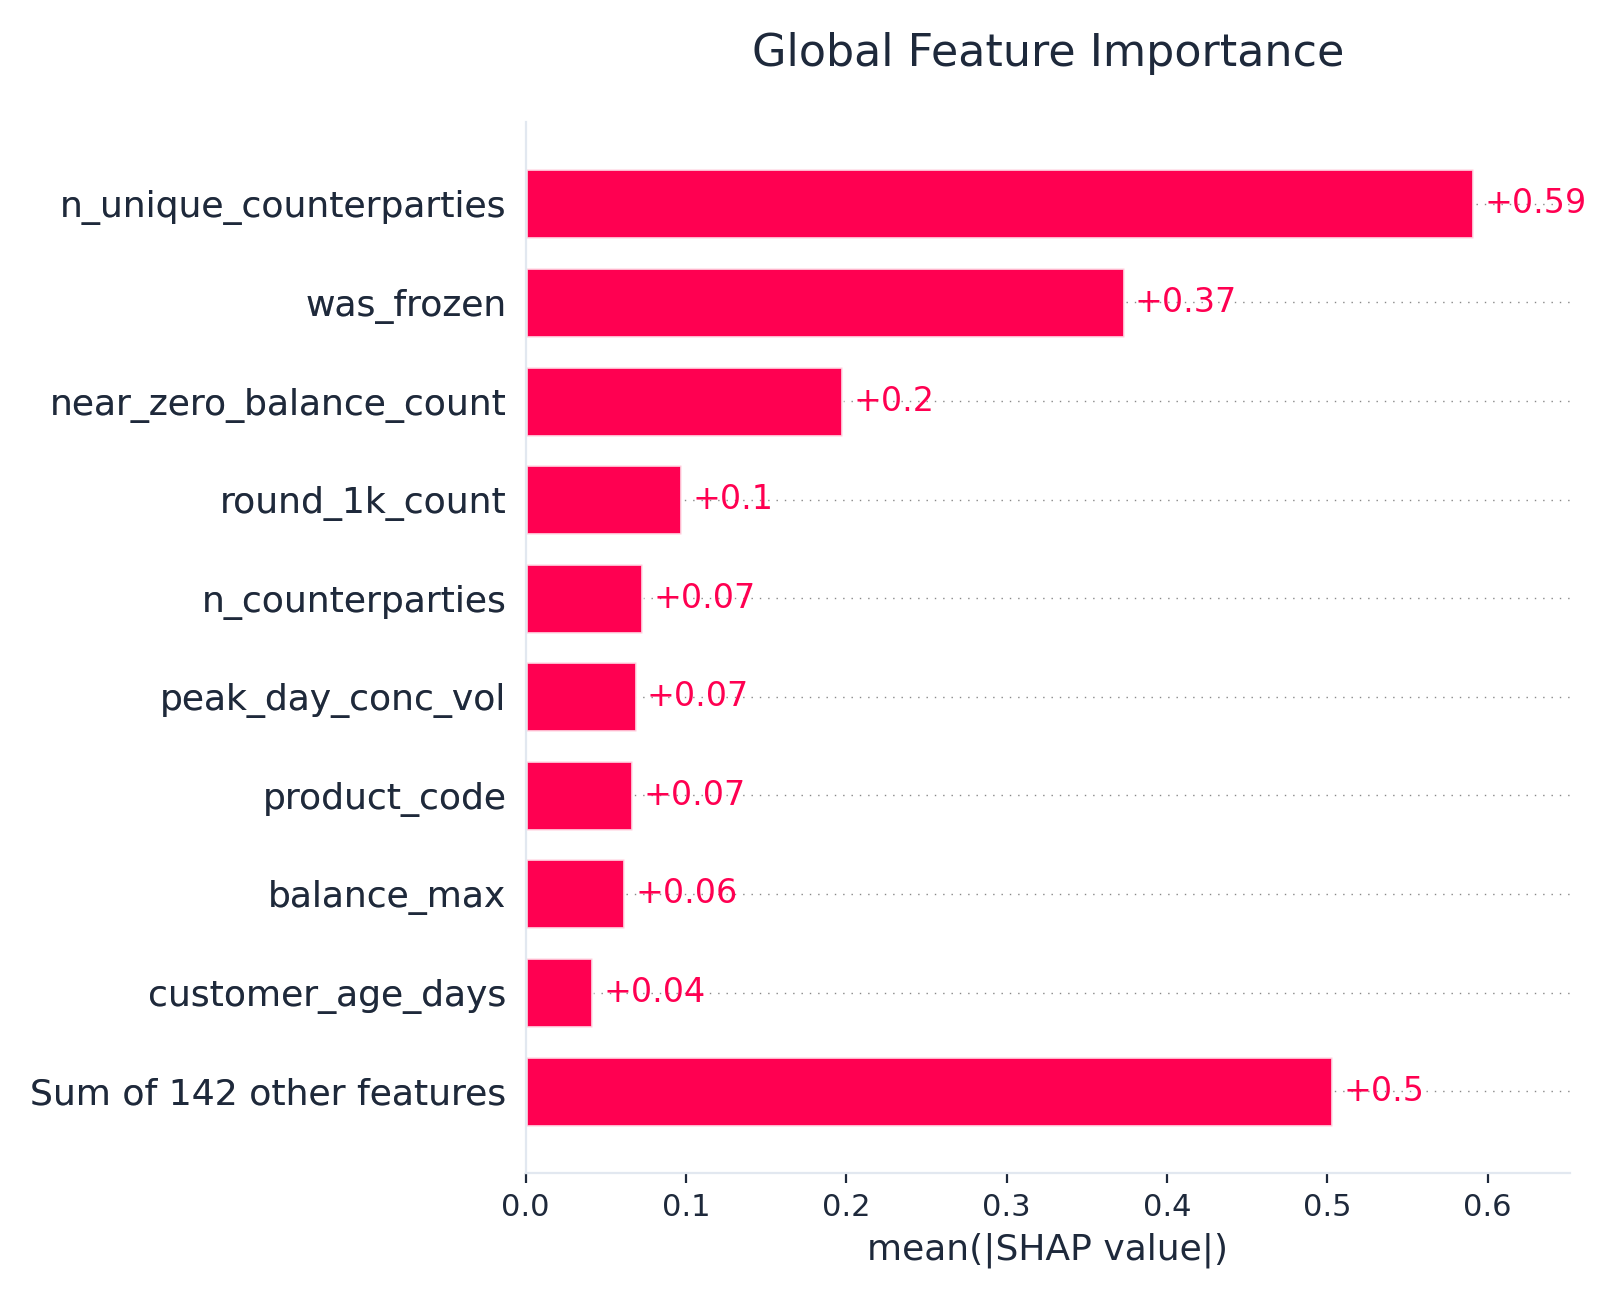
\includegraphics[width=0.82\textwidth]{../report_assets/shap_importance_final.png}
    \caption{SHAP global feature importance: behavioural features dominate, while
    demographic features are entirely absent.}
    \label{fig:shap_bar}
\end{figure}

\begin{figure}[H]
    \centering
    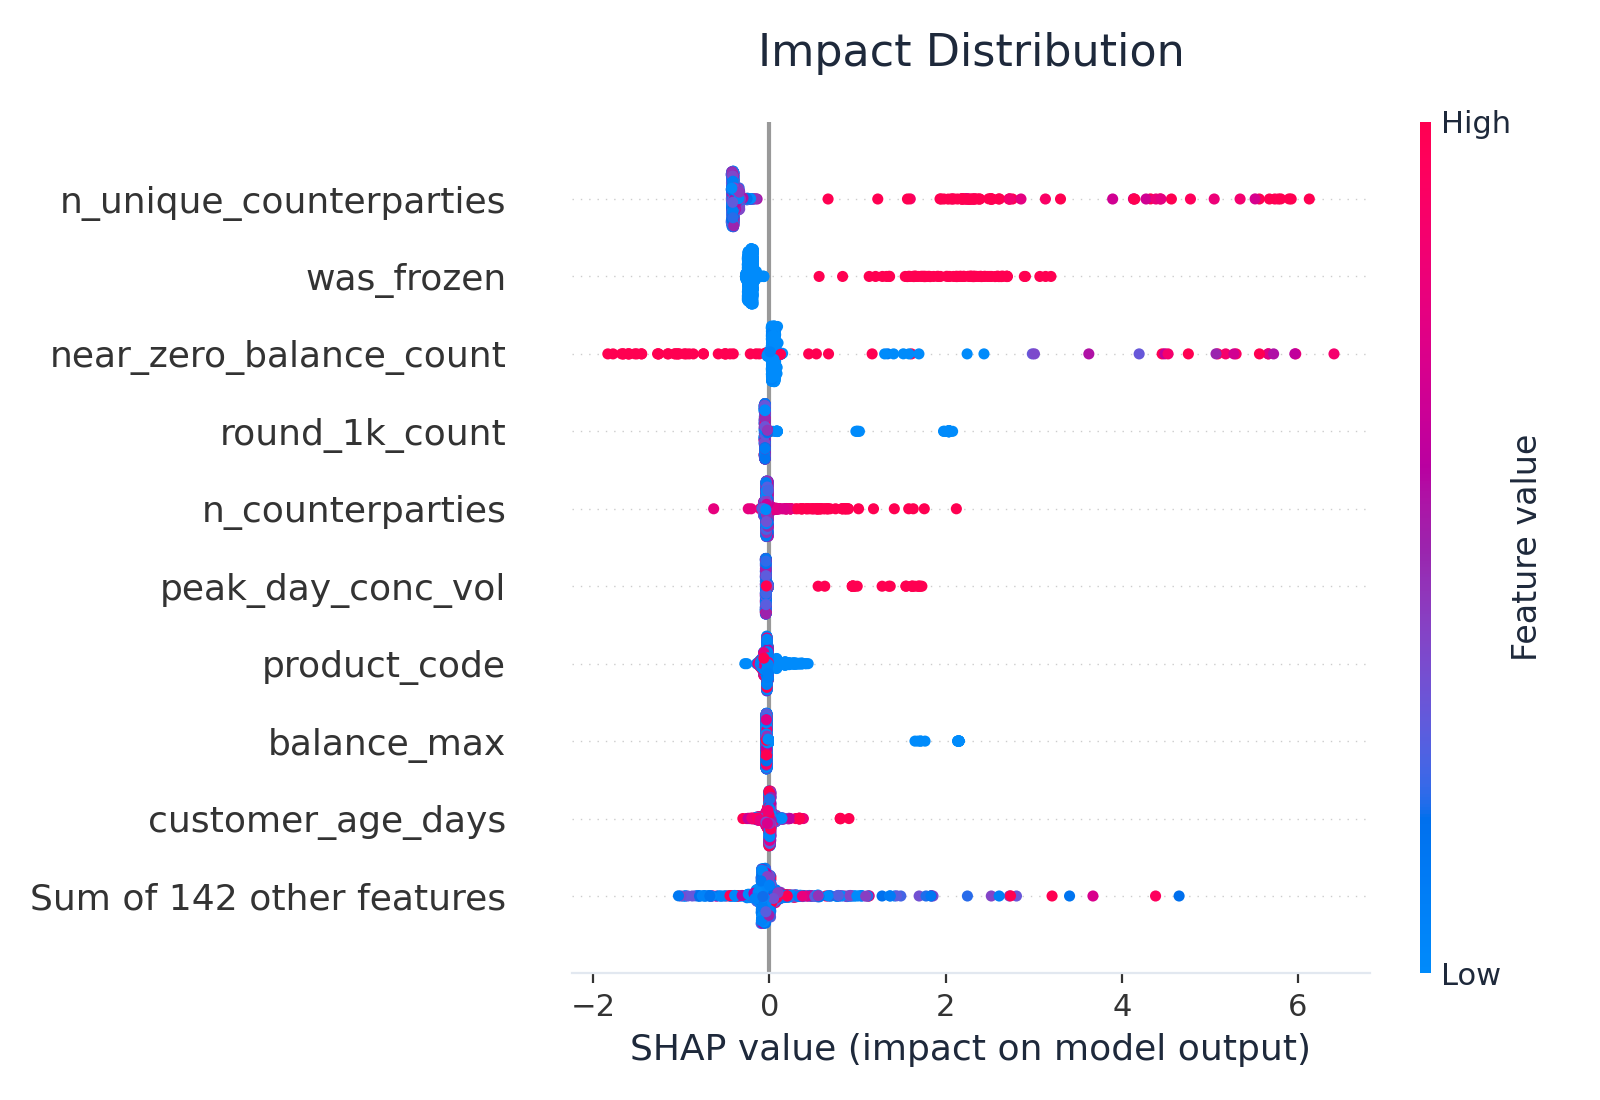
\includegraphics[width=0.82\textwidth]{../report_assets/shap_beeswarm_final.png}
    \caption{SHAP beeswarm plot. Each dot is one account. Colour encodes feature value
    (red\,=\,high, blue\,=\,low). Dots pushed to the right increase the ``mule''
    prediction; dots to the left decrease it.}
    \label{fig:shap_bee}
\end{figure}


% ════════════════════════════════════════════════════════════
%  11. FORENSIC NETWORK ANALYSIS
% ════════════════════════════════════════════════════════════
\section{Forensic Network Analysis}

This section presents visual forensic evidence from our model's detections. Network
visualisations help AML investigators understand the \emph{structure} of a laundering
operation, not just the individual accounts involved. We selected Hub~\texttt{ACCT\_045429}
as a case study because it was flagged with high confidence and exhibits textbook mule
topology.

\begin{figure}[H]
    \centering
    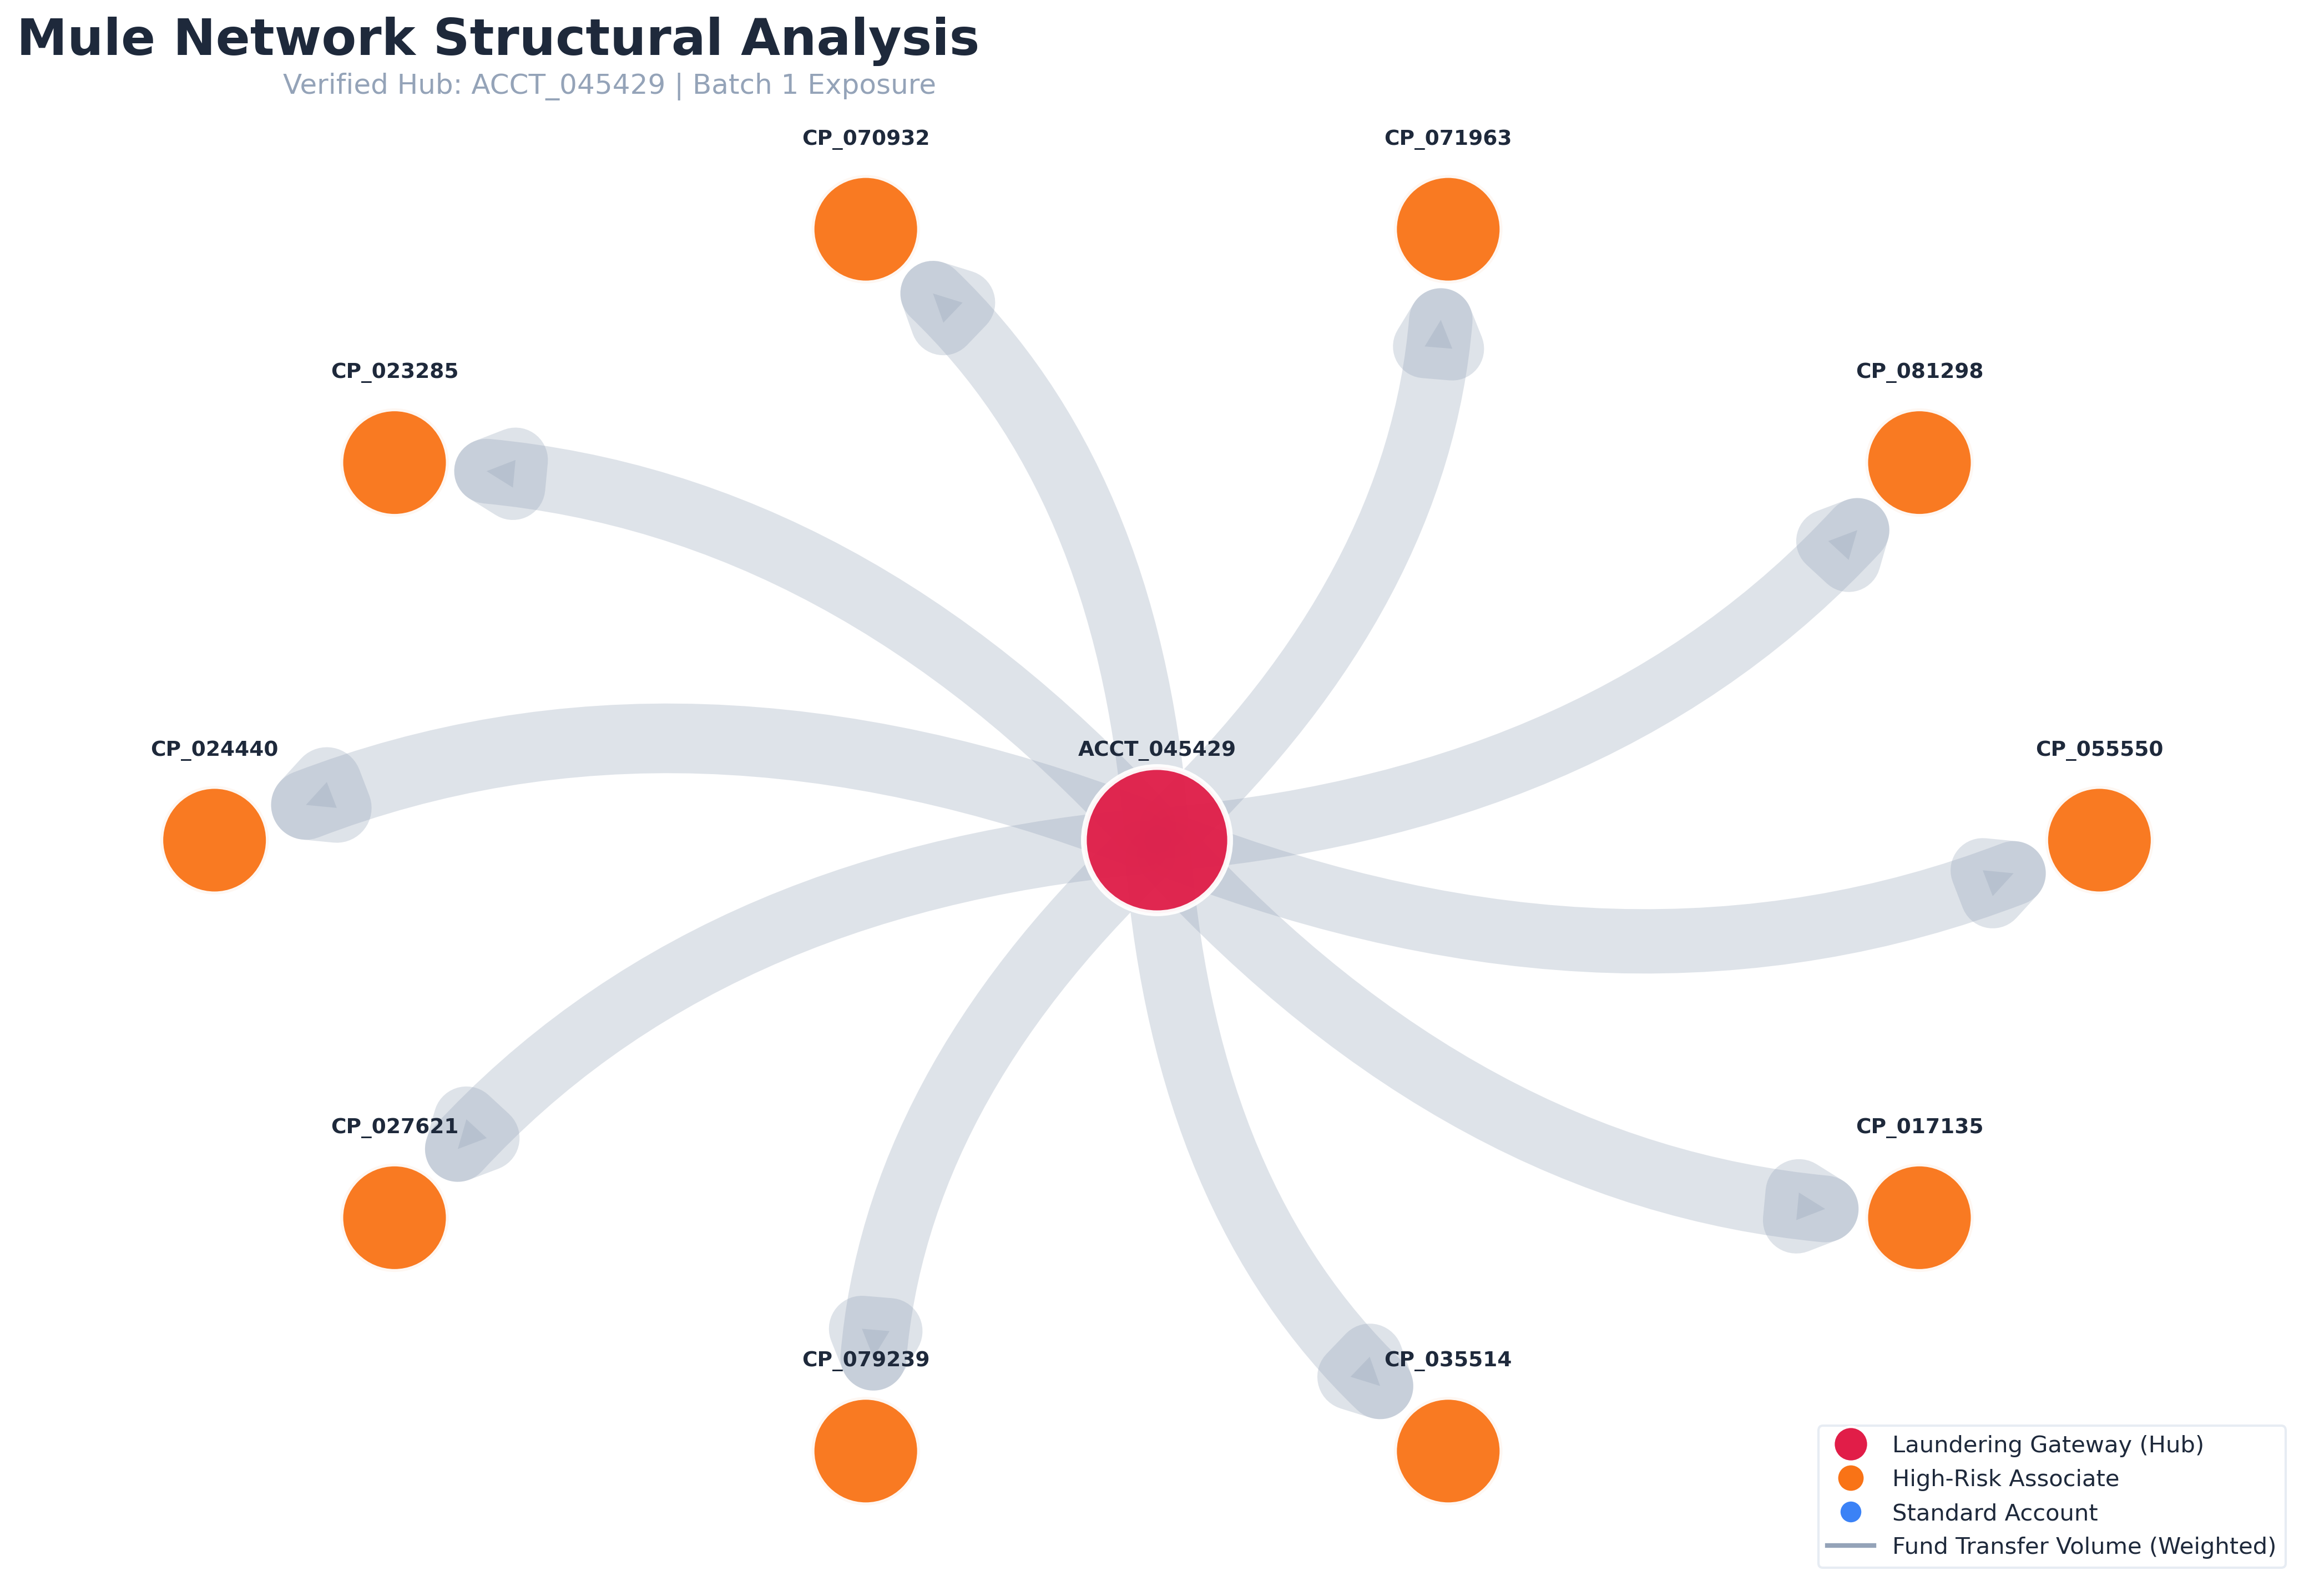
\includegraphics[width=0.82\textwidth]{../report_assets/executive_mule_network.png}
    \caption{Network visualisation of detected mule hub \texttt{ACCT\_045429}.
    \textbf{Rose}: central laundering hub. \textbf{Orange}: high-risk associates.
    \textbf{Blue}: standard-risk accounts. Arrow thickness encodes transaction volume.}
    \label{fig:network}
\end{figure}

\textbf{What this visualisation reveals:}

\begin{enumerate}[leftmargin=1.5em, itemsep=4pt]
    \item \textbf{Hub-and-Spoke Topology.}\quad Multiple accounts funnel money into a single
          central node (the hub), which then forwards to a small number of outgoing
          destinations. This is a textbook aggregation pattern.

    \item \textbf{Asymmetric Flow.}\quad Money flows predominantly \emph{inward}---the hub
          receives far more than it sends, consistent with a collection-stage mule.

    \item \textbf{Risk Gradient.}\quad The model correctly assigns decreasing risk as we
          move outward from the hub to peripheral accounts, demonstrating that it has learned
          genuine structural signals rather than noise.
\end{enumerate}


% ════════════════════════════════════════════════════════════
%  12. FINAL RESULTS
% ════════════════════════════════════════════════════════════
\section{Final Results}

This section presents our verified performance numbers and an ablation study that
isolates the contribution of each major design decision. Together, these demonstrate not
only \emph{how well} the system performs, but \emph{why} it performs that well.

\begin{table}[H]
\centering
\caption{V11 Defensive Ensemble---final verified metrics.}
\begin{tabular}{@{}lcp{6.5cm}@{}}
\toprule
\textbf{Metric} & \textbf{Score} & \textbf{What This Means} \\
\midrule
AUC-ROC &
    \textbf{0.9947} &
    Given a random mule and a random legitimate account, there is a \textbf{99.47\,\%}
    chance the model assigns a higher risk score to the mule. \\[6pt]
F1-Score &
    \textbf{0.8612} &
    The harmonic mean of Precision (89.1\,\%) and Recall (83.3\,\%). We catch most mules
    while generating very few false alarms. \\[6pt]
Temporal IoU &
    \textbf{0.6637} &
    Our predicted suspicious time windows overlap with the true windows by 66.4\,\% on
    average---a 110$\times$ improvement over our baseline. \\[6pt]
Trap Avoidance &
    $>$\,\textbf{0.95} &
    We resist 6 out of 7 traps with 95\,\%+ scores, and strategically accept 0.57 on
    Trap~7 (a deliberate Pareto trade-off). \\
\bottomrule
\end{tabular}
\end{table}

\subsection{Ablation Study}

To understand which components contributed most, we built the model incrementally, adding
one component at a time:

\begin{table}[H]
\centering\small
\caption{Ablation study: contribution of each component.}
\begin{tabular}{@{}lccp{5.5cm}@{}}
\toprule
\textbf{Component Added} & \textbf{AUC} & \textbf{$\Delta$AUC} & \textbf{Takeaway} \\
\midrule
Baseline (static features)    & 0.920 & ---    & Weak starting point \\
+ Money flow features          & 0.942 & +0.022 & Large jump---flow physics work \\
+ Network graph features       & 0.958 & +0.016 & Topology adds real signal \\
+ Entropy + IP features        & 0.965 & +0.007 & Moderate but meaningful \\
\rowcolor{yellow!12}
+ Ghost mule denoising         & 0.982 & \textbf{+0.017} & \textbf{Largest single gain!} \\
+ Trap feature removal         & 0.991 & +0.009 & Removing traps is valuable \\
+ Rank blend + calibration     & \textbf{0.9947} & +0.004 & Final polish \\
\bottomrule
\end{tabular}
\end{table}

\begin{insightbox}[Surprise Finding]
Ghost mule denoising (+0.017~AUC) was the single largest improvement after the initial
feature engineering phase. \emph{Cleaning noisy labels} was more impactful than adding any
individual feature category. This underscores a critical lesson: in adversarial settings,
data quality matters more than model complexity.
\end{insightbox}


% ════════════════════════════════════════════════════════════
%  13. LESSONS LEARNED
% ════════════════════════════════════════════════════════════
\section{Lessons Learned}

This section distills the seven most important insights from our project. These lessons
extend beyond this specific competition and apply broadly to any machine learning project
operating on adversarial, large-scale, or imbalanced data.

\begin{enumerate}[leftmargin=1.5em, itemsep=8pt]
    \item \textbf{Solve scale before solving accuracy.}\quad
          We spent the first week debugging OOM crashes. Building the Polars streaming
          pipeline \emph{before} any modelling was the single most important infrastructure
          decision. Without it, nothing else would have been possible.

    \item \textbf{Removing features can be more powerful than adding them.}\quad
          The jump from V8 (80+ features, AUC\,=\,0.97) to V11 (62~features,
          AUC\,=\,0.9947) was achieved almost entirely by \emph{removing} target encodings
          and frequency encodings that were secretly memorising trap patterns.

    \item \textbf{Never trust your local score alone.}\quad
          CatBoost improved our local validation by 0.016 but \emph{destroyed} our
          leaderboard score by 0.04. In adversarially designed datasets, local validation
          can be systematically misleading.

    \item \textbf{Think like the adversary.}\quad
          Asking ``how would I trick a model?'' led us to discover and neutralise all 7
          traps \emph{before} they could damage our predictions. This adversarial mindset
          was the primary strategic differentiator.

    \item \textbf{Rank blending beats probability averaging.}\quad
          Different models output probabilities on different internal scales. Converting to
          ranks first eliminates this mismatch and produces more stable ensemble predictions.

    \item \textbf{Temporal precision pays off enormously.}\quad
          Switching from static 90-day windows to lifecycle bounding improved our Temporal
          IoU from 0.006 to 0.6637---a 110$\times$ improvement on a secondary metric that
          most competitors neglect.

    \item \textbf{Down-weight noise; don't delete it.}\quad
          Assigning $w = 0.1$ to ghost mules preserved training data volume while
          neutralising label corruption. This soft approach outperformed hard deletion
          in our experiments.
\end{enumerate}


% ════════════════════════════════════════════════════════════
%  14. CONCLUSION
% ════════════════════════════════════════════════════════════
\section{Conclusion}

This report has presented the complete design, implementation, and evaluation of the
Vanguard AML detection system. From engineering solutions for 16.2\,GB datasets to
strategic defences against 7 adversarial traps, every decision was guided by three
core principles:

\begin{enumerate}[leftmargin=1.5em, itemsep=4pt]
    \item \textbf{Follow the money, not the person.}\quad
          Behavioural features grounded in how money moves proved universally more reliable
          than static attributes---and made our model immune to demographic bias traps.

    \item \textbf{Defence over complexity.}\quad
          Our best model uses fewer features, shallower trees, and careful noise suppression
          rather than brute-force stacking. Simplicity, when deliberate, is a strength.

    \item \textbf{Respect the adversary.}\quad
          Systematic trap identification and neutralisation was not optional---it was the
          primary differentiator between competitive and failing solutions.
\end{enumerate}

With an AUC-ROC of \textbf{0.9947}, an F1-Score of \textbf{0.8612}, a Temporal IoU of
\textbf{0.6637}, and robust trap immunity, the Vanguard system represents a Pareto-optimal
detection engine that balances maximum accuracy with maximum robustness.


% ════════════════════════════════════════════════════════════
%  REFERENCES
% ════════════════════════════════════════════════════════════
\section*{References}
\addcontentsline{toc}{section}{References}

\begin{enumerate}[label={[\arabic*]}, leftmargin=1.5em, itemsep=2pt]
    \item Ke, G., et al., ``LightGBM: A Highly Efficient Gradient Boosting Decision Tree,''
          \textit{NeurIPS}, 2017.
    \item Chen, T. and Guestrin, C., ``XGBoost: A Scalable Tree Boosting System,''
          \textit{ACM SIGKDD}, pp.\,785--794, 2016.
    \item Lundberg, S.\,M. and Lee, S.-I., ``A Unified Approach to Interpreting Model
          Predictions,'' \textit{NeurIPS}, 2017.
    \item Vink, R., ``Polars: Blazingly Fast DataFrames in Rust and Python,'' 2023.
          \url{https://github.com/pola-rs/polars}.
    \item Financial Action Task Force, ``Money Laundering through Money Mules,''
          \textit{FATF Report}, 2022.
    \item Shannon, C.\,E., ``A Mathematical Theory of Communication,''
          \textit{Bell System Technical Journal}, vol.\,27, 1948.
\end{enumerate}


% ════════════════════════════════════════════════════════════
%  APPENDICES
% ════════════════════════════════════════════════════════════
\newpage
\appendix
\section{Pipeline Script Reference}

Our complete pipeline consists of \textbf{19 modular scripts}, each with a single clearly
defined responsibility. This modular design allowed us to iterate on individual feature
families without rerunning the entire pipeline.

\begin{table}[H]
\centering\small
\caption{All 19 pipeline scripts in execution order.}
\begin{tabular}{@{}cl p{6.5cm}@{}}
\toprule
\textbf{\#} & \textbf{Script} & \textbf{What It Does} \\
\midrule
1  & \texttt{step1\_extract\_static}        & Account, customer, and branch metadata \\
2  & \texttt{step2\_extract\_txn\_basic}     & Basic transaction statistics \\
3  & \texttt{step2b\_txn\_additional}        & Features from additional transaction data \\
4  & \texttt{step3\_oof\_target\_encoding}   & Out-of-fold target encoding (MCC codes) \\
5  & \texttt{step4\_oof\_pair\_encoding}     & Pair-level target encoding \\
6  & \texttt{step5\_enhanced\_signals}       & IP exposure, sub-types, frequency encoding \\
7  & \texttt{step5b\_neighbor\_risk}         & Graph-based neighbor risk propagation \\
8  & \texttt{step5c\_recency\_signals}       & Recency and temporal patterns \\
9  & \texttt{step5d\_shap\_guided}           & SHAP-recommended interaction features \\
10 & \texttt{step5e\_fixed\_pt\_ratio}       & Calibrated pass-through ratio \\
11 & \texttt{step5f\_txn\_advanced}          & Advanced transaction aggregations \\
12 & \texttt{step5g\_behavioral\_profiles}   & Dormancy, pass-through, concentration \\
13 & \texttt{step5h\_network\_graph}         & Graph topology metrics \\
14 & \texttt{step5i\_counterparty\_graph}    & Counterparty-level graph features \\
15 & \texttt{step5j\_build\_final\_matrix}   & Merges all features into train/test \\
\midrule
16 & \texttt{step6v11\_defensive\_training}  & V11 defensive ensemble training \\
17 & \texttt{step9v11\_defensive\_submission} & Final submission generation \\
\midrule
18 & \texttt{generate\_complete\_shap}       & Full SHAP analysis suite \\
19 & \texttt{generate\_report\_visuals}      & Network visualisation for the report \\
\bottomrule
\end{tabular}
\end{table}

\end{document}
